\documentclass[portrait,a0b,posterdraft]{a0poster}
\usepackage{german,epsf,pstricks}
\usepackage{graphicx}
\usepackage{subcaption}
\usepackage{forloop}


\begin{document}

\begin{figure}
\begin{subfigure}{.1\textwidth}
\centering
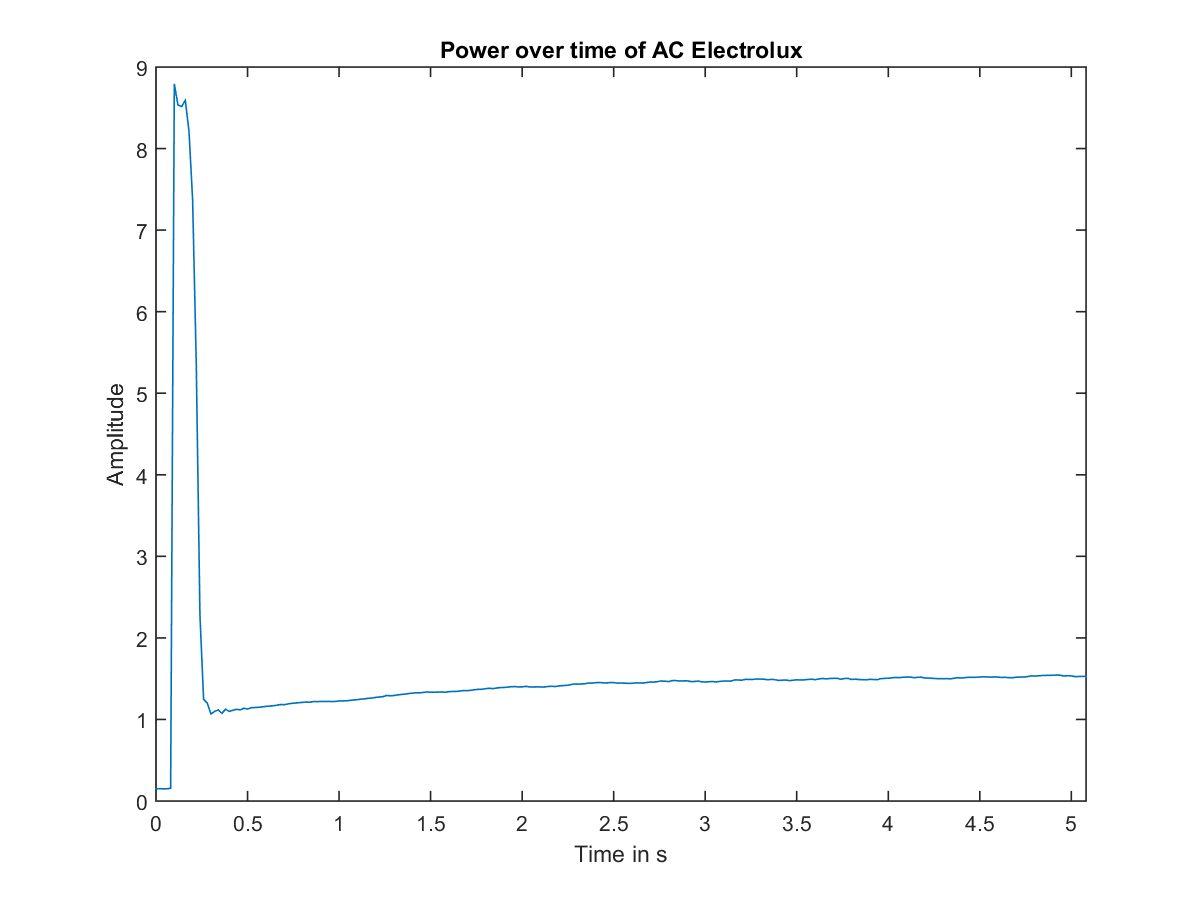
\includegraphics[width=\linewidth]{AC_Electrolux_powerTimeDomain.png}
\caption{spectrogram}
\end{subfigure}
\begin{subfigure}{.1\textwidth}
\centering
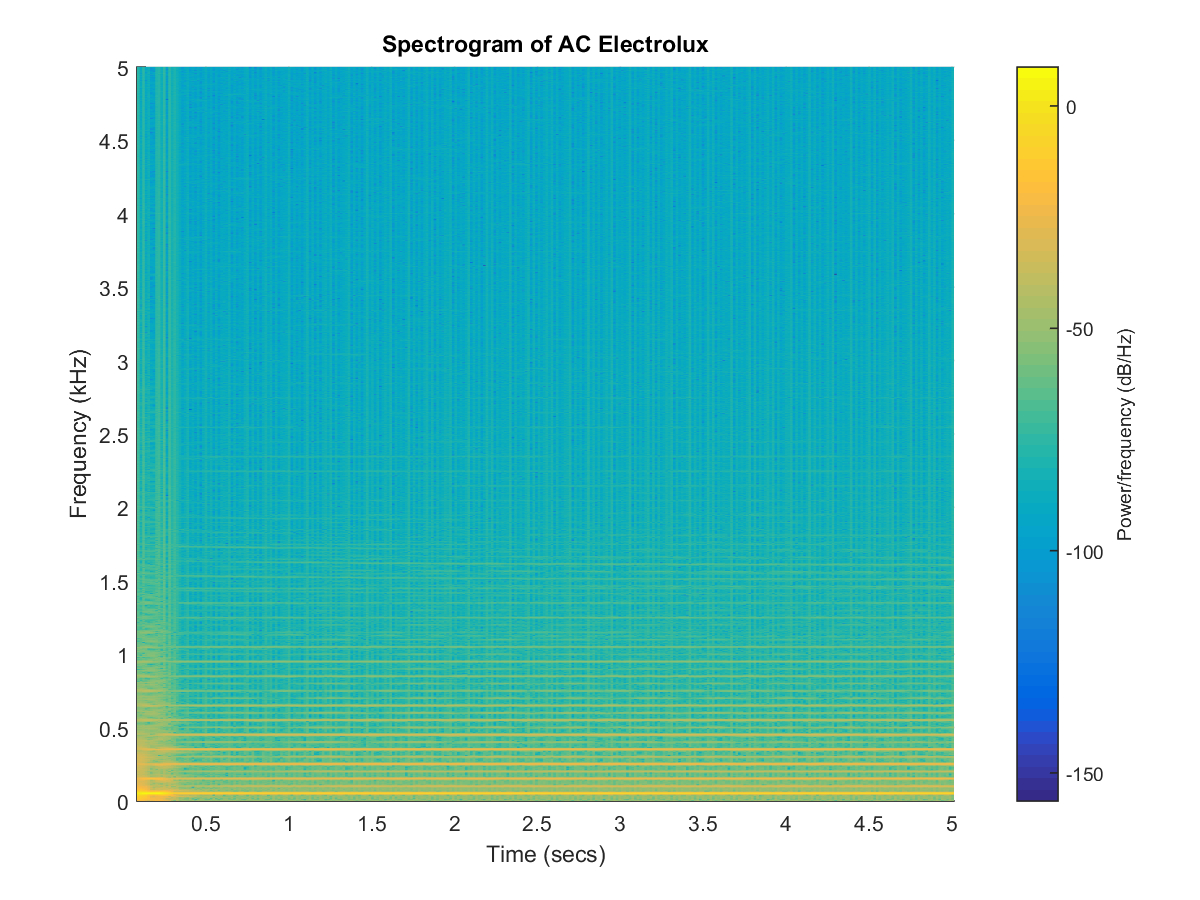
\includegraphics[width=\linewidth]{AC_Electrolux_spectrogram.png}
\caption{spectrum}
\end{subfigure}
\begin{subfigure}{.1\textwidth}
\centering
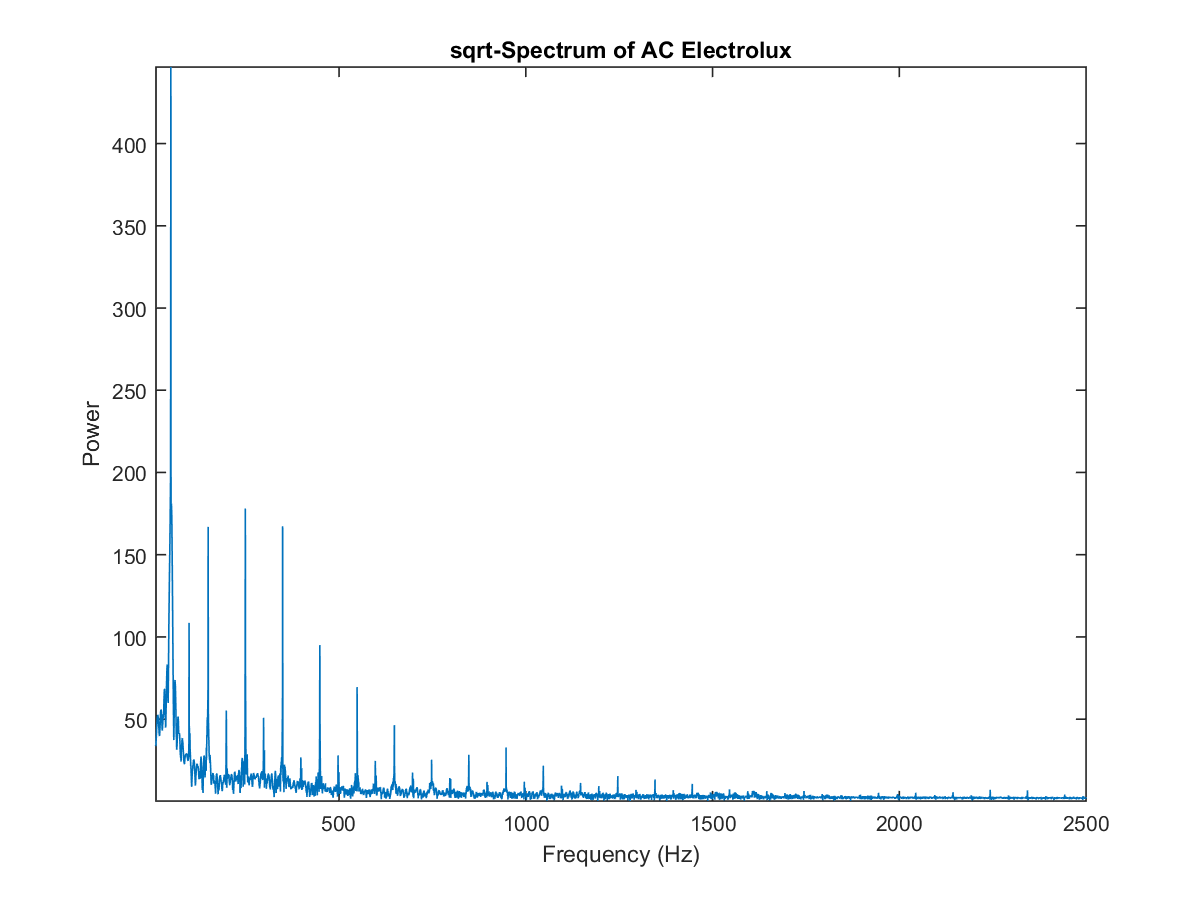
\includegraphics[width=\linewidth]{AC_Electrolux_spectrum.png}
\caption{spectrogram}
\end{subfigure}
\begin{subfigure}{.1\textwidth}
\centering
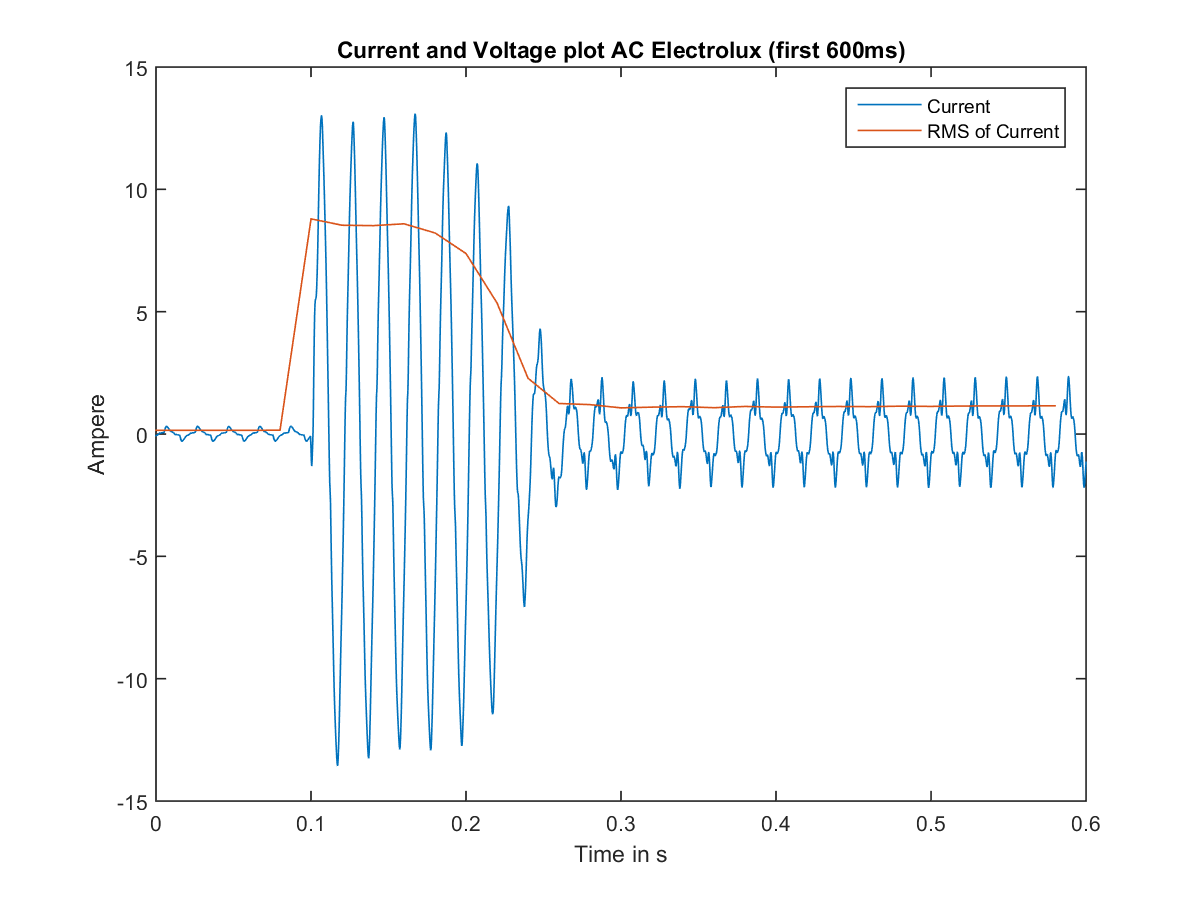
\includegraphics[width=\linewidth]{AC_Electrolux_timeDomainShort.png}
\caption{spectrum}
\end{subfigure}
\begin{subfigure}{.1\textwidth}
\centering
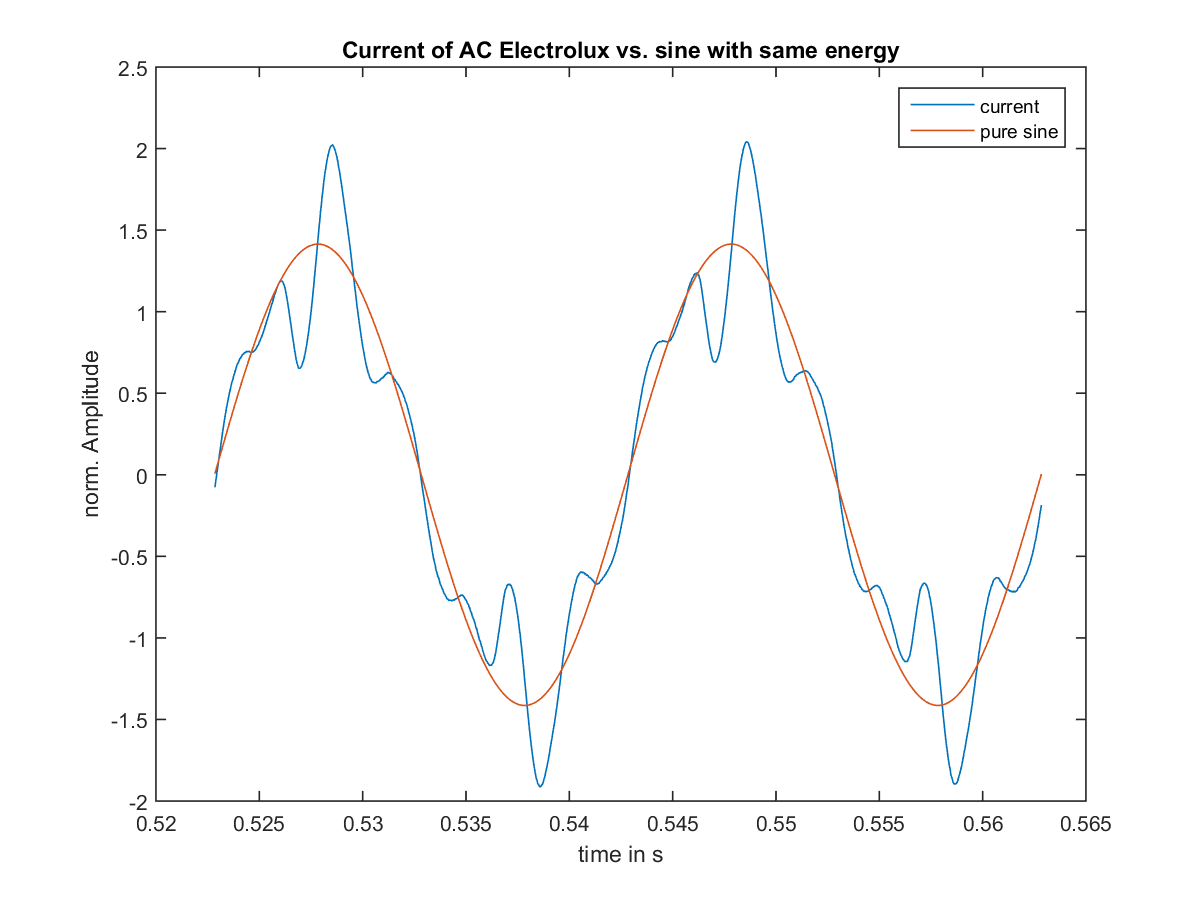
\includegraphics[width=\linewidth]{AC_Electrolux_waveform.png}
\caption{spectrum}
\end{subfigure}
\end{figure}

\newcounter{ct}
\forloop{ct}{1}{\value{ct} < 5}%
{
Appliance: AC Electrolux
\begin{figure}
\begin{subfigure}{.1\textwidth}
\centering
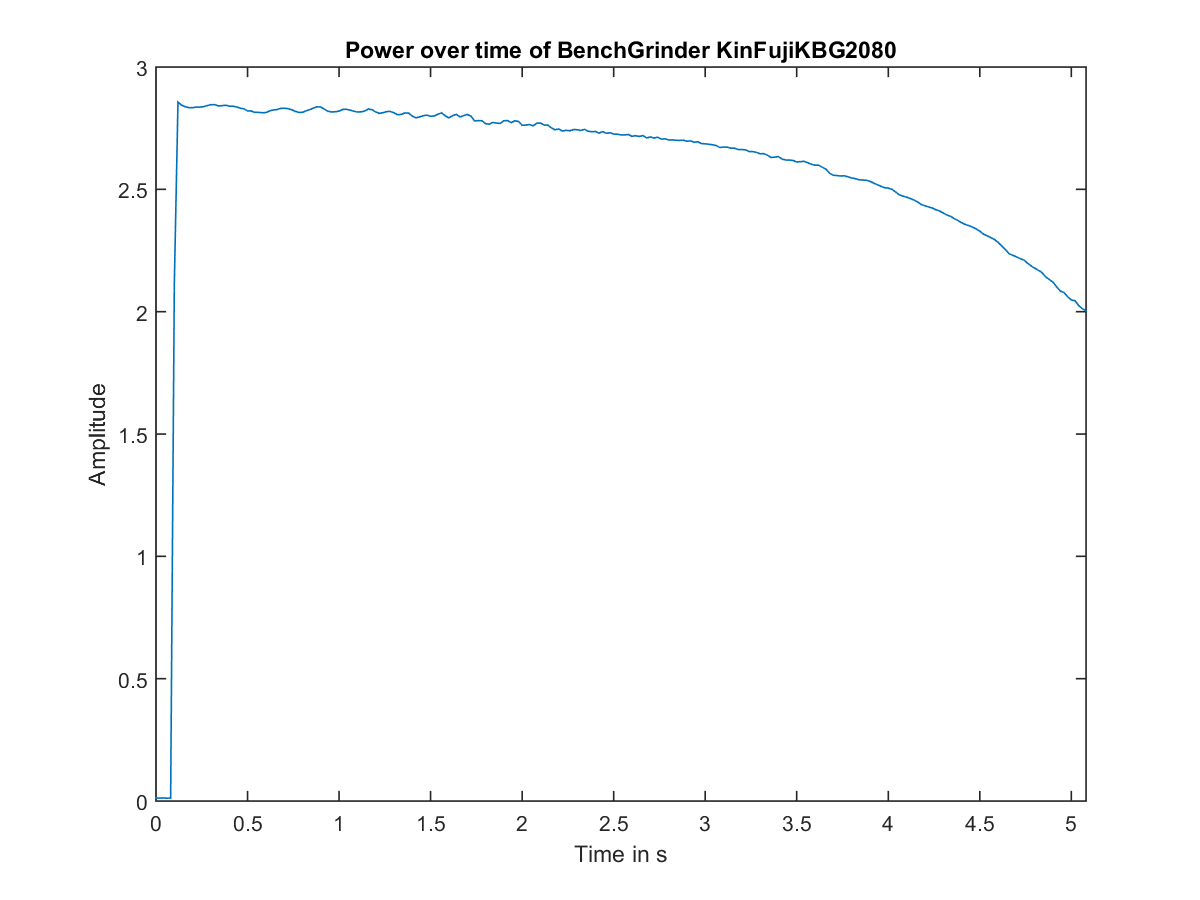
\includegraphics[width=\linewidth]{BenchGrinder_KinFujiKBG2080_powerTimeDomain.png}
\caption{spectrogram}
\end{subfigure}
\begin{subfigure}{.1\textwidth}
\centering
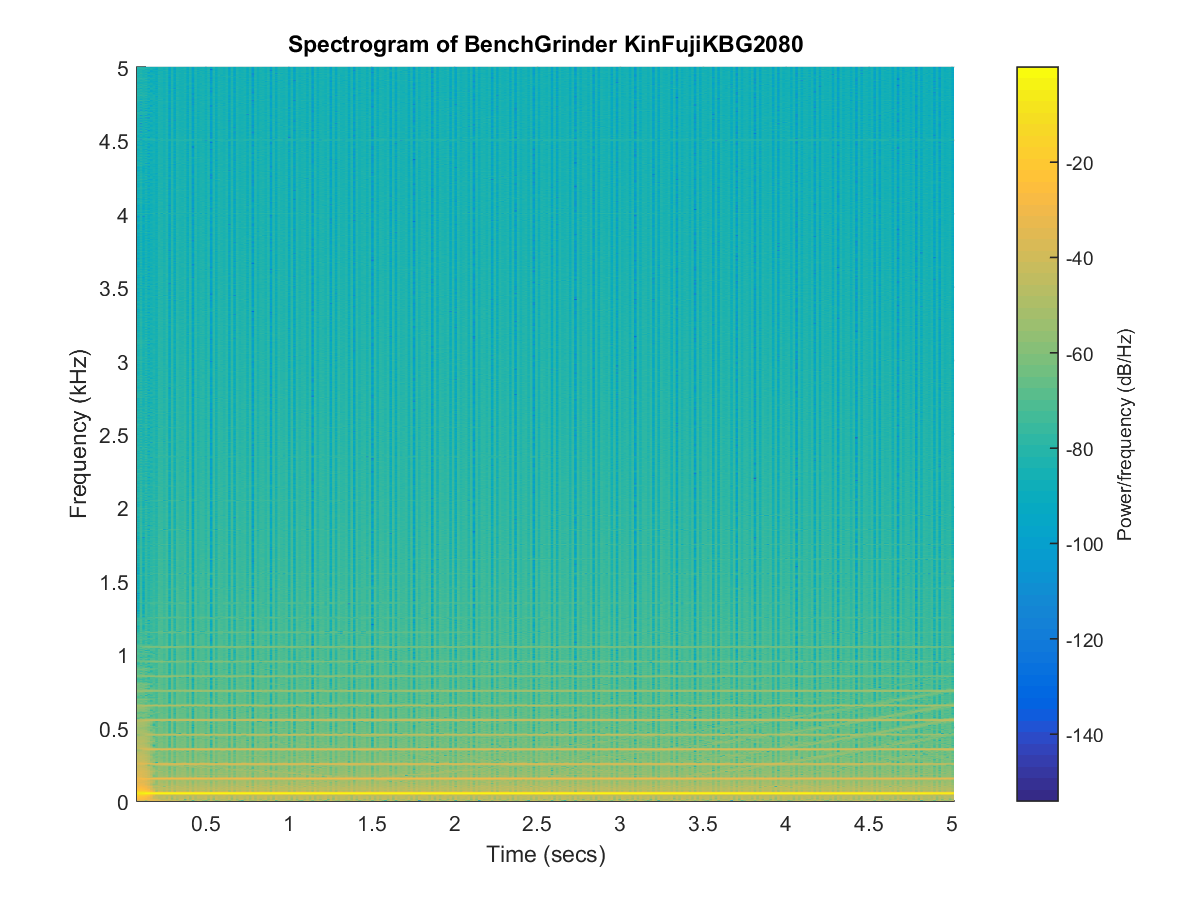
\includegraphics[width=\linewidth]{BenchGrinder_KinFujiKBG2080_spectrogram.png}
\caption{spectrum}
\end{subfigure}
\begin{subfigure}{.1\textwidth}
\centering
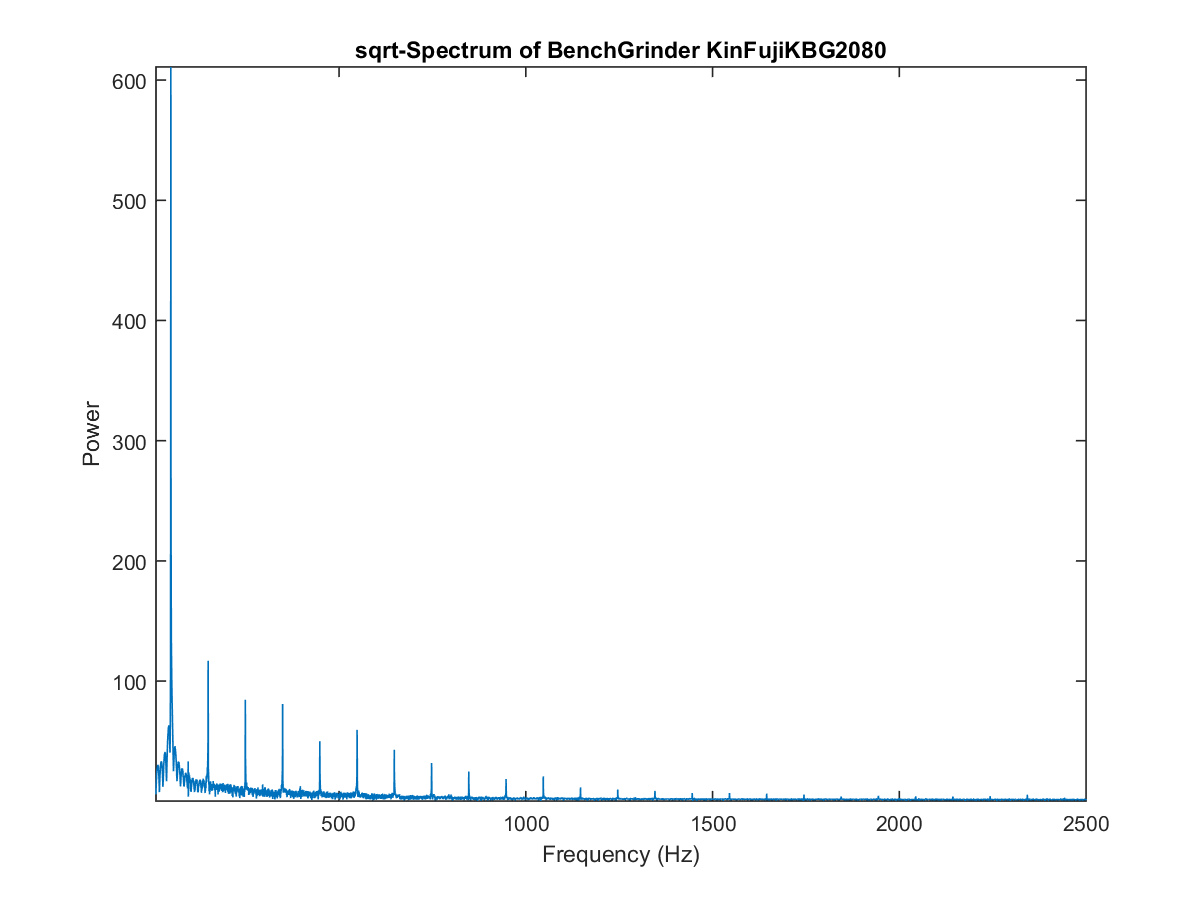
\includegraphics[width=\linewidth]{BenchGrinder_KinFujiKBG2080_spectrum.png}
\caption{spectrogram}
\end{subfigure}
\begin{subfigure}{.1\textwidth}
\centering
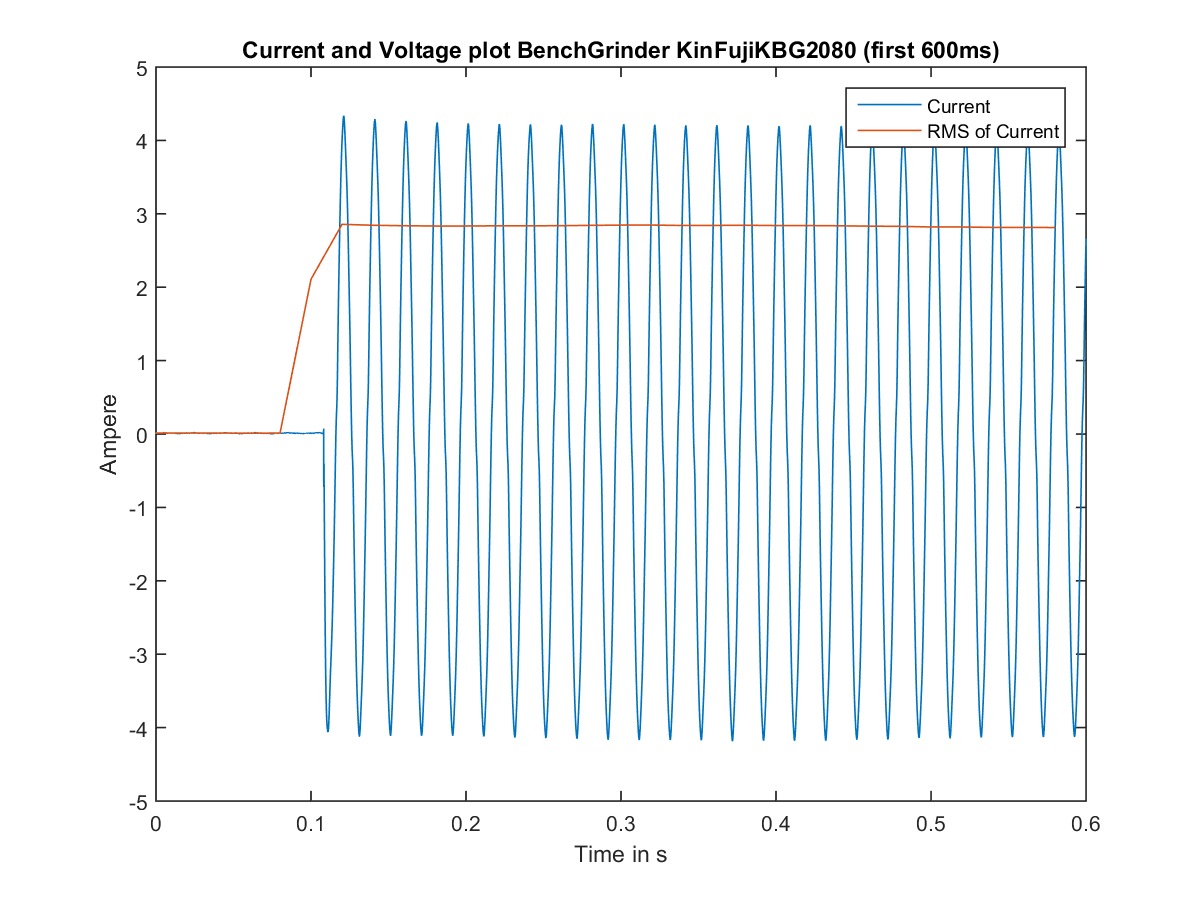
\includegraphics[width=\linewidth]{BenchGrinder_KinFujiKBG2080_timeDomainShort.png}
\caption{spectrum}
\end{subfigure}
\begin{subfigure}{.1\textwidth}
\centering
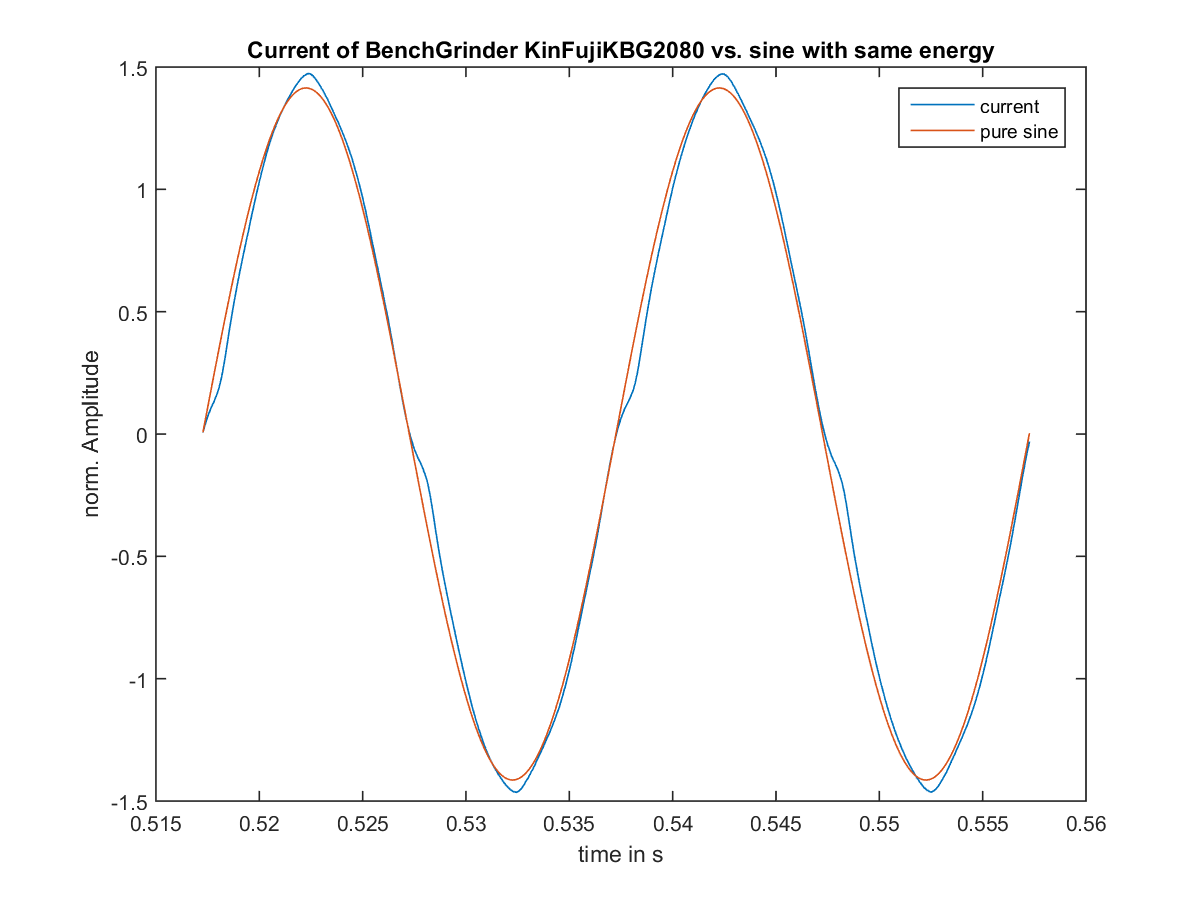
\includegraphics[width=\linewidth]{BenchGrinder_KinFujiKBG2080_waveform.png}
\caption{spectrum}
\end{subfigure}
\end{figure}
}


%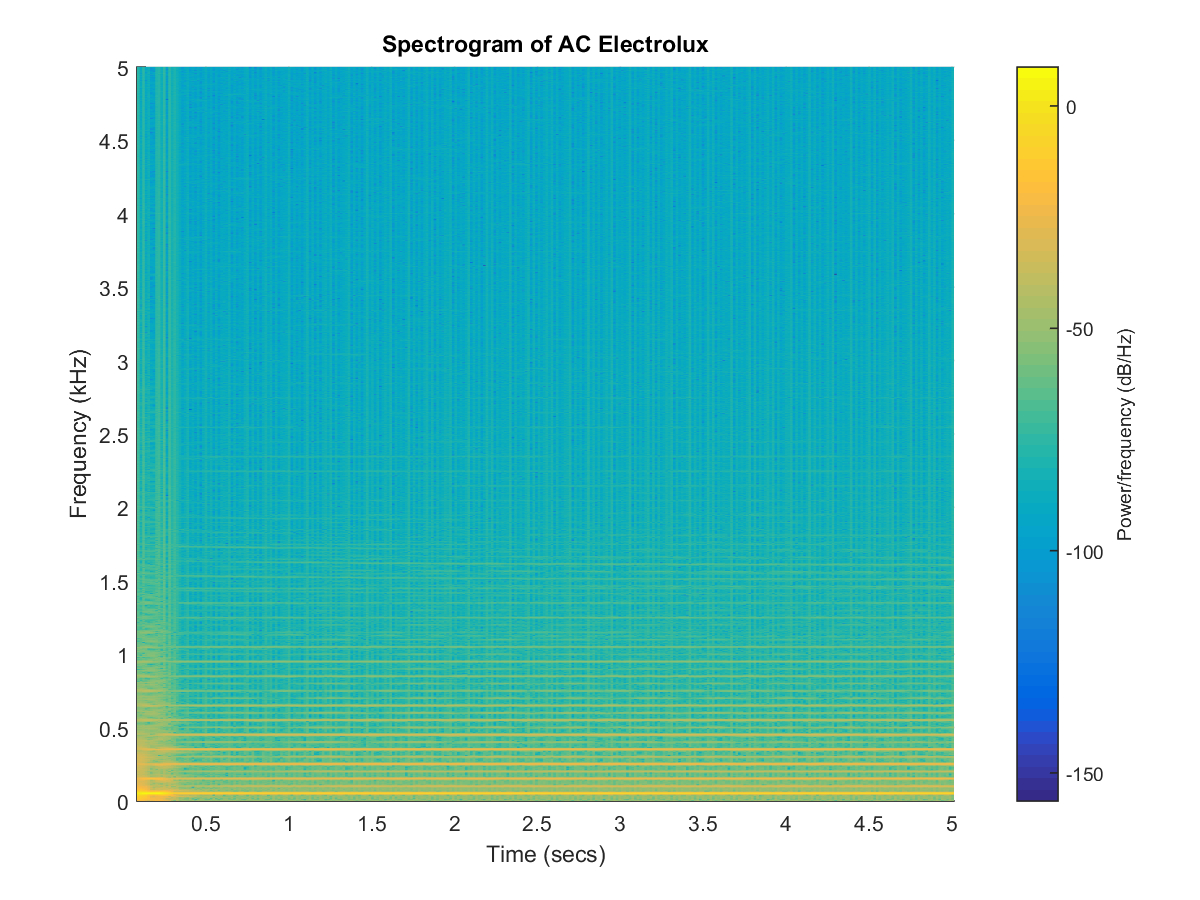
\includegraphics{AC_Electrolux_spectrogram.png}

\end{document}
